\chapter{Exigences non fonctionnelles}
Dans ce chapitre, les différentes exigences non fonctionnelles qui ont été sélectionnées seront explicitées. Pour rappel, de telles exigences décrivent les propriétés que le produit doit respecter. Pour ce faire, plusieurs de ces qualités ont été sélectionnées dans le modèle de Volere et seront présentées ci-dessous.

\section{Ergonomie et convivialité du produit}
SportEasy étant destiné à être une application sur smartphone, les couleurs, les interfaces et tout ce qui touche au visuel seront les premières choses que percevront les utilisateurs. Il est donc plus qu'important de définir quelque chose de plaisant et d'agréable afin de tout de suite accrocher le potentiel sportif et gagner le pas sur la concurrence. Afin de maximiser l'expérience de l'utilisateur et les chances de survie de l'application, il faut que les interfaces respectent certaines contraintes et que le packaging du produit soit attrayant.

\subsection*{Interface}
Cette application a pour vocation de configurer des séances sportives pour des utilisateurs aguerris ou non, comme il l'a déjà été mentionné plusieurs fois plus haut dans ce travail. Dès lors, il est nécessaire que son emploi soit rapide et intuitif et ne nécessite pas de lectures fastidieuses. Dès lors, il est important que la majorité de l'application soit graphique et compréhensible en un coup d'\oe il.\\

\'Etant donné que l'étude de partenariat n'a été menée que dans le cadre de la Belgique, notamment en Wallonie, il est normal que les interfaces soient définies, dans un premier temps, en français. Cependant, afin de toucher plus de monde, il est nécessaire de traduire ces interfaces le plus vite possible dans des langues plus accessibles (l'anglais, principalement, afin de devenir rapidement international).\\

La Figure \ref{fig:interfaces} montre des prototypes d'interfaces (qui ont d'ailleurs été plus détaillés dans le chapitre précédent). Ces IHM sont en accord avec la vision que le produit doit avoir : simples, sobres et efficaces.

\begin{figure}[!h]
	\centering
	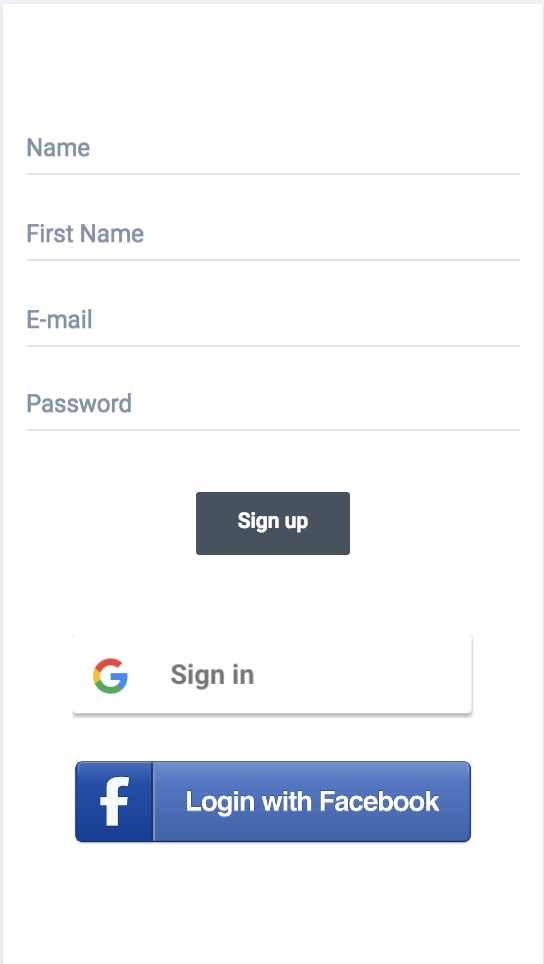
\includegraphics[scale=0.3]{ihms/inscription}
	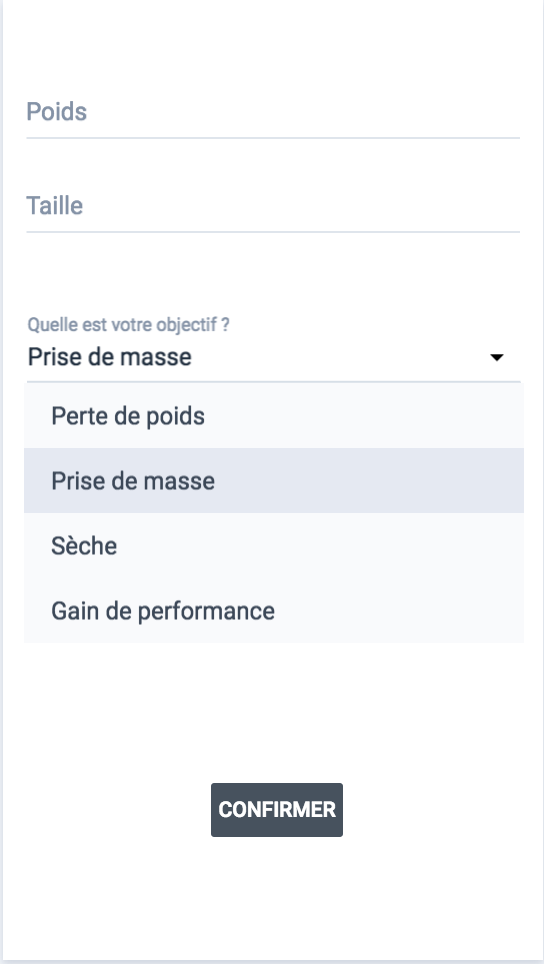
\includegraphics[scale=0.3]{ihms/caracteristiques}
	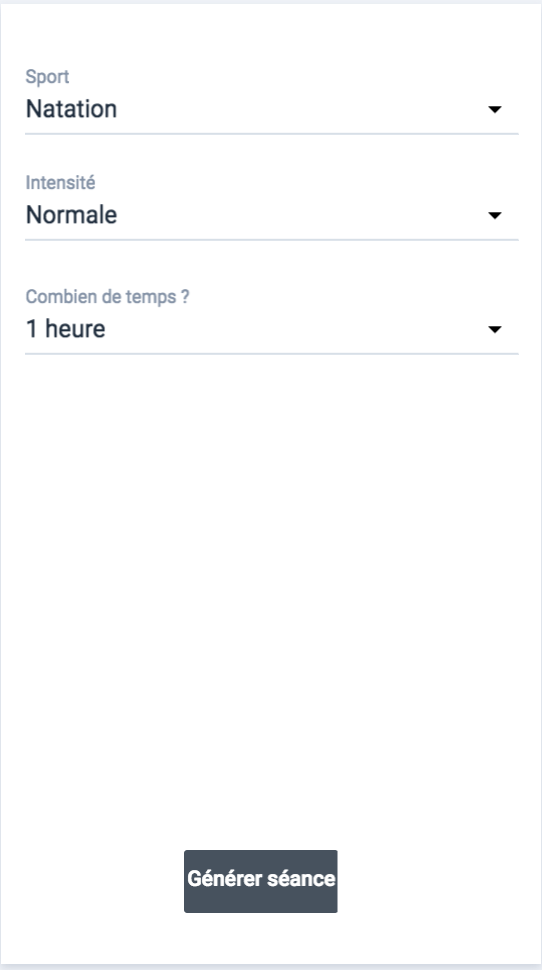
\includegraphics[scale=0.3]{ihms/seance}
	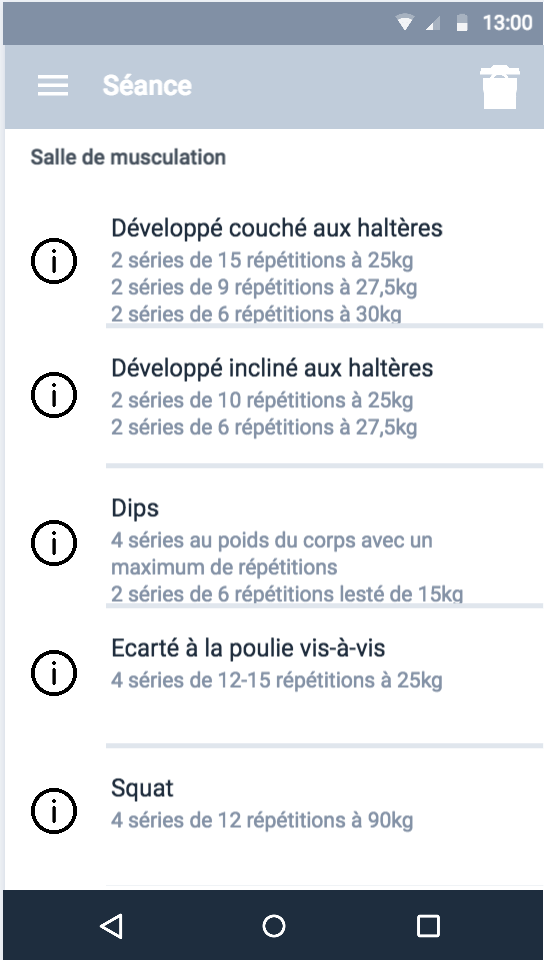
\includegraphics[scale=0.3]{ihms/normal_session}
	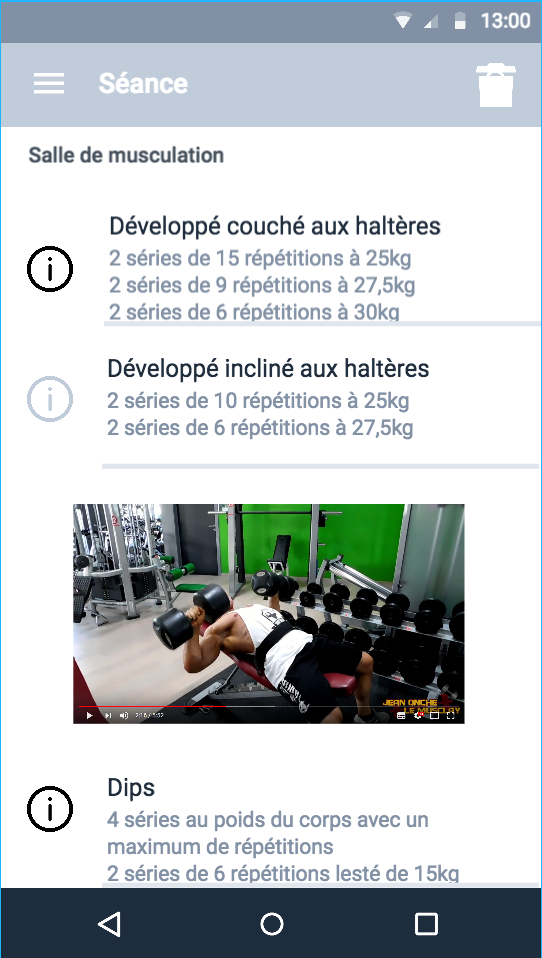
\includegraphics[scale=0.3]{ihms/get_information_about_exo}
	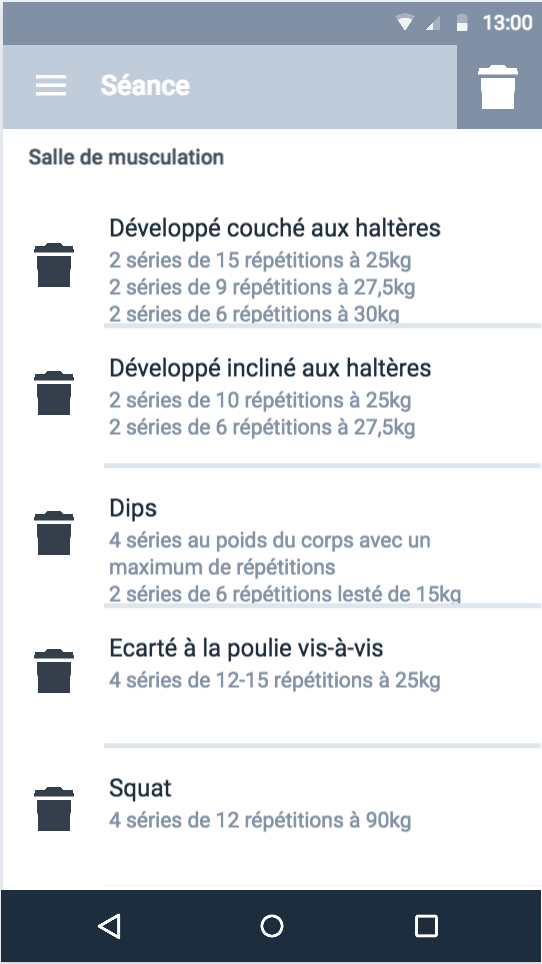
\includegraphics[scale=0.3]{ihms/remove_exo}
	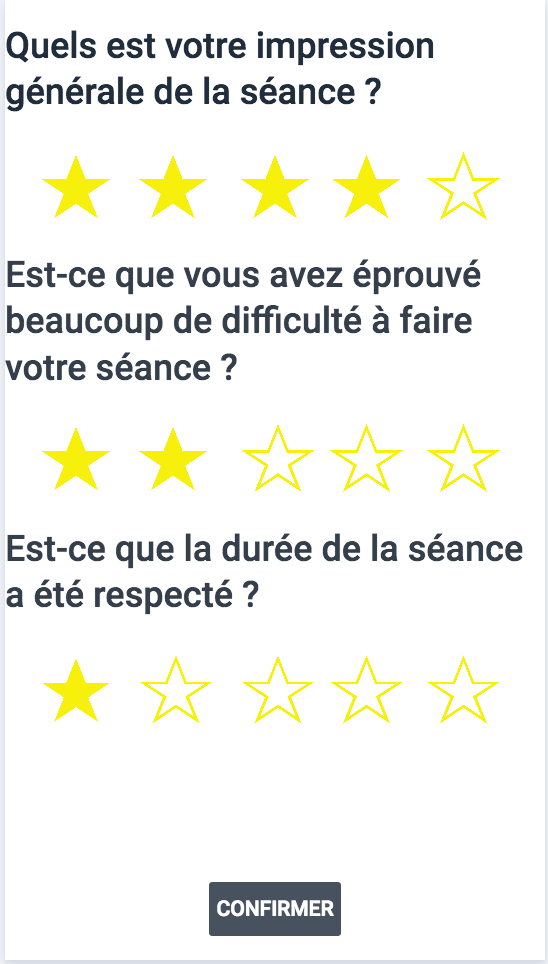
\includegraphics[scale=0.3]{ihms/rating_before_update}
	\caption{\label{fig:interfaces}Interfaces}
\end{figure}

\subsection*{Style et packaging du produit}
S'il est difficilement envisageable de définir un packaging pour une application mobile, il est néanmoins primordial que le produit respecte quelques conditions de style afin d'être un succès une fois lancé sur le marché.\\

Ainsi, le produit doit avoir l'air moderne et dynamique. Il est donc nécessaire que ce dernier respecte les dernières tendances en matière d'applications mobiles afin de se frayer un chemin aisé sur le marché et ne pas être désuet avant même d'avoir existé.\\

De même, bien que l'application soit destinée à toute personne souhaitant faire du sport, elle touchera rarement les enfants, qui nécessitent une attention particulière dans leur séance sportive de part leur croissance toujours bien active. Dès lors, l'application ne doit pas présenter de couleurs particulièrement \og flashy \fg{}.\\

Enfin, il est important que le produit suscite l'envie de faire du sport et stimule la motivation de l'utilisateur. Pour se faire, il doit employer un design frais, dynamique et énergétique tout en étant présenté de façon motivante. Le tout est que l'utilisateur ait envie de se lever pour faire du sport à peine ayant eu accès à l'application.

\section{Facilité d'utilisation et facteurs humains}
Le produit étant destiné à être utilisé par des personnes, non formées pour l'occasion, il est important de définir des exigences d'utilisation ; notamment la facilité d'emploi et d'apprentissage.

\subsection*{Facilité d'utilisation}
Les fonctionnalités du produit devraient être très simples. Comme mentionné précédemment, l'utilisateur souhaitant démarrer une séance de sport ne veut pas perdre 30 minutes de son temps à la configurer, ce qui lui laisserait effectivement moins de temps pour faire un entrainement. Dès lors, les points suivants doivent être respectés :\\

\begin{itemize}
	\item \textbf{Efficacité de la prise en main :} l'utilisateur doit être capable de prendre en main l'application et d'en utiliser toutes les fonctionnalités très rapidement. Dès lors, la prise en main sera plus longue (didacticiel d'emploi) et des pré-réglages seront stockés pour que la prise en main soit très rapide. Dès lors, après les 20 premières minutes d'utilisation de l'application, l'utilisateur est supposé savoir utiliser cette dernière parfaitement et rapidement.\\
	
	\item \textbf{Facilité de mémorisation :} l'application est supposée être intuitive pour être utilisée directement, sans besoin de formation particulière. Dès lors, il est considéré que l'utilisateur devrait être capable de se remémorer l'emploi d'une fonctionnalité après la 1\iere{} utilisation. Cependant, le produit étant destiné à des personnes de tout âge et de tout milieu, la limite sera fixée pour 3 utilisations de chaque fonctionnalité pour être certain que l'utilisateur se souvienne bien comment chaque fonctionnalité s'emploie.\\
	
	\item \textbf{Taux d'erreur :} l'utilisateur peut commettre des erreurs, cependant cela risque d'influencer en mal ses performances et donc biaiser l'application et sa fonctionnalité à proposer des séances adaptées. Ainsi, il existe 3 types d'erreurs, classées de bénignes à \og grave \fg{}. La première, c'est de se tromper dans la configuration de sa séance de sport. Il faut alors couper l'application et la relancer, cela fait perdre son temps à l'utilisateur. La seconde est le fait de se tromper dans le feedback fournit à la fin de la séance. Bien qu'il est rare de rencontrer ce cas, s'il se produit, l'adaptation de la séance ne sera pas efficace. Enfin, l'utilisateur peut couper l'application avant d'avoir terminé et validé sa séance. Dans ce cas, l'application ne pourra mettre à jour ses données et se comporter de façon efficace pour les prochains entrainements, ce qui est déplorable. Dès lors, il est nécessaire que le taux d'erreur global ne dépasse pas les 5\% en 1 mois d'utilisation afin de ne pas entacher le comportement normal du produit.\\
	
	\item \textbf{Satisfaction globale :} grâce aux feedbacks fournis par les fournisseurs d'applications mobiles (Play Store, Apple Store, ...), il est aisé de mesurer la satisfaction globale de l'utilisateur. Dès lors, il est important que l'application ne descende pas en dessous d'une satisfaction générale de 80\% endéans des 6 premiers mois.
\end{itemize}

\subsection*{Facilité d'apprentissage}
Comme expliqué ci-avant, le produit doit être facilement utilisable afin que l'utilisateur ne perde pas du temps précieux pour le configurer. De même, il faut tenir compte du fait que l'utilisateur normal est un adulte lambda qui ne doit présenter aucune qualification particulière pour employer l'application. Ainsi, un didacticiel sera mis en place afin que toute personne capable de lire puisse comprendre les étapes nécessaires à la configuration de la séance.\\

Très vite, le public doit être capable d'employer le produit sans devoir chercher. Au bout de 3 utilisations (répétition des mêmes mouvements), l'utilisateur doit être capable de configurer sa séance en toute maîtrise en 5 minutes maximum.

\subsection*{Facilité de compréhension et politesse}
Le produit n'est pas destiné à un professionnel du sport. Cela signifie qu'un amateur, un novice, peut souhaiter l'employer afin de s'entrainer. S'il connait certains termes techniques, tous les sens lui échappent sûrement. Cependant, il ne serait pas professionnel d'employer un vocabulaire infantile à la place. Pour s'assurer de la compréhension du vocabulaire sportif, des schémas ou vidéos explicatifs doivent être disponibles si l'utilisateur clique sur un des exercices.\\

Par ailleurs, il est aussi primordial de cacher les détails d'implémentation et de s'assurer qu'aucune exception n'apparaitra à l'utilisateur en tant que telle, dans un langage \og hérétique \fg{}. Toute exception devra être transformée en un message d'erreur clair et concis dans la langue de l'utilisateur.

\section{Fonctionnement du produit}
Ce chapitre traite des performances du produit quant à diverses données.


%- Rapidité et temps de latence
%- Sécurité
%- Précision et exactitude
%- Fiabilité et disponibilité
%- Robustesse et tolérance à un emploi erroné
%- Capacité de stockage et montée en charge
%- Adaptation du produit à une augmentation de volume à gérer
%- Longévité

\section{Adéquation du produit avec son environnement}
- Environnement physique
- Environnement technologique
- Applications "partenaires" (collaboration)
- Commercialisation

\section{Maintenance et support du produit}
- Maintenance
- Conditions spéciales de la maintenance
- Exigences en matière de support
- Exigences de portabilité
- Installation du système

\section{Sécurité}
- Accès au système
- Intégrité
- Protection des données à caractère personnel
- Audit et traçabilité
- Protection contre les infections

\section{Exigences culturelles et politiques}
- Exigences culturelles
- Exigences politiques

\section{Lois et standards}
- Conformité avec la loi
- Conformité avec des standards